\documentclass[problem]{mcs}

\begin{pcomments}
\pcomment{PS_more_numbered_trees}
\pcomment{from S08, ps9; f07.ps9;prob4 edited by ARM 11/14/09}
\pcomment{solution can and should be explained more simply --ARM 11/14/09}
\end{pcomments}

\pkeywords{
 multinomial_coefficient
 numbered_trees
 bijection
 degree_of_a_vertex
}

%%%%%%%%%%%%%%%%%%%%%%%%%%%%%%%%%%%%%%%%%%%%%%%%%%%%%%%%%%%%%%%%%%%%%
% Problem starts here
%%%%%%%%%%%%%%%%%%%%%%%%%%%%%%%%%%%%%%%%%%%%%%%%%%%%%%%%%%%%%%%%%%%%%

\begin{problem}

  The \term{degree sequence} of a simple graph is the weakly
  decreasing sequence of degrees of its vertices.  For example, the
  degree sequence for the 5-vertex numbered tree pictured in the
  Figure~\bref{codetrees} in Problem~\bref{CP_numbered_trees} is
  $(2,2,2,1,1)$ and for the 7-vertex tree it is $(3,3,2,1,1,1,1)$.

\inhandout{
\begin{figure}[htb]
\begin{center}
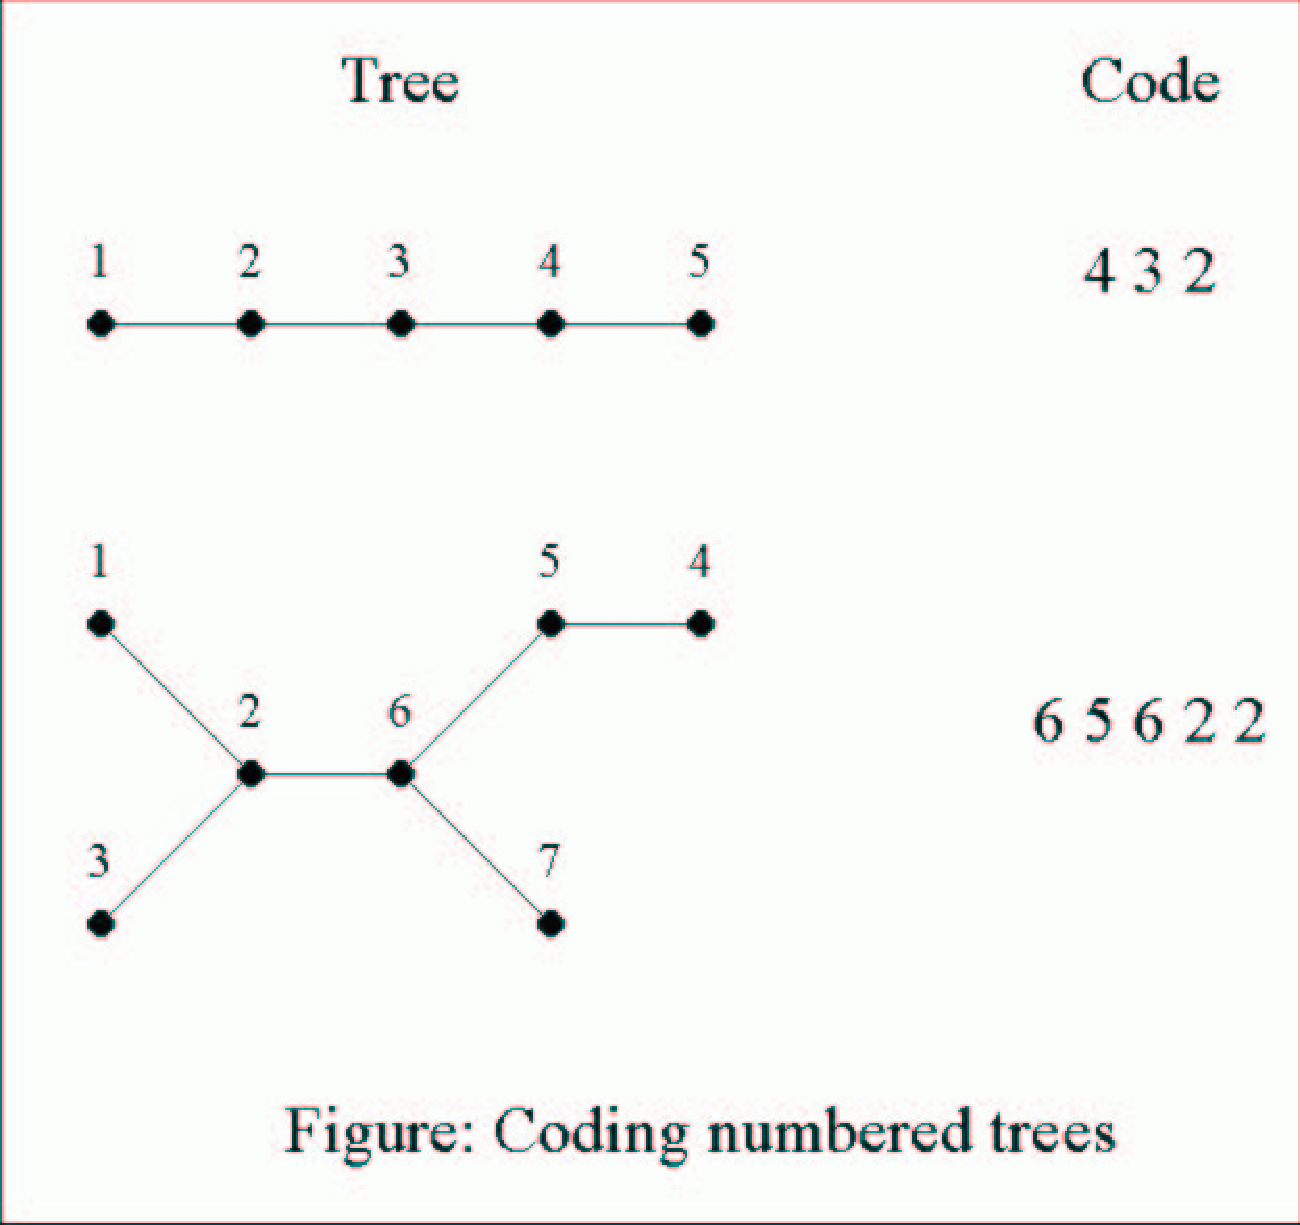
\includegraphics[width=4in]{n-2}
\end{center}
\caption{}
\label{codetrees}
\end{figure}
}


We're interested in counting how many \idx{numbered trees} there are
with a given degree sequence.  We'll do this using the \idx{bijection}
defined in Problem~\bref{CP_numbered_trees} between $n$-vertex
numbered trees and length $n-2$ code words whose characters are
integers between $1$ and $n$.

\iffalse
This bijective coding of trees to code words is reviewed in
the box below.

\textbox{
\begin{center}
\large \textbf{Numbered Tree Codes}
\end{center}

An $n$-vertex \term{numbered tree} is a tree whose vertex set is
$\set{1,2,\dots,n}$ for some $n > 2$.  We define the \emph{code} of
the numbered tree to be a sequence of $n-2$ integers from 1 to $n$
obtained by the following recursive process:
\begin{quotation}
  If there are more than two vertices left, write down the \emph{father}
  of the largest leaf\footnote{The necessarily unique node adjacent to a
    leaf is called its \term{father}.}, delete this \emph{leaf}, and
  continue this process on the resulting smaller tree.
  If there are only two vertices left, then stop ---the code is complete.
\end{quotation}
For example, the codes of a couple of numbered trees are shown in the Figure~\ref{codetrees}.


}
\fi

The \emph{occurrence number} for a character in a word is the number of
times that the character occurs in the word.  For example, in the word
\texttt{65622}, the occurrence number for \texttt{6} is two, and the
occurrence number for \texttt{5} is one.  The \emph{occurrence sequence}
of a word is the weakly decreasing sequence of occurrence numbers of
characters in the word.  The occurrence sequence for this word is
$(2,2,1)$ because it has two occurrences of each of the characters
\texttt{6} and \texttt{2}, and one occurrence of \texttt{5}.

\bparts
\ppart\label{occnum}

There is simple relationship between the degree sequence of an $n$-vertex
numbered tree and the occurrence sequence of its code.  Describe this
relationship and explain why it holds.  Conclude that counting $n$-vertex
numbered trees with a given degree sequence is the same as counting the
number of length $n-2$ code words with a given occurrence sequence.

\hint How many times does a vertex of degree, $d$, occur in the code?

\begin{solution}
  A vertex of degree $d$ appears in the code $d-1$ times.  Consequently,
  if the degree sequence of a numbered tree has the form
  $(d_1,d_2,\dots,d_k,1,\dots,1)$ where $d_k>1$, then the occurrence
  sequence of its code is $(d_1-1,d_2-1,\dots,d_k-1)$.  Since the
  correspondence between numbered trees and code words is a bijection, the
  number of numbered trees with degree sequence
  $(d_1,d_2,\dots,d_k,1,\dots,1)$ is the same as the number of code words
  with occurrence sequence $(d_1-1,d_2-1,\dots,d_k-1)$.

  To see why a vertex of degree $d$ appears in the code $d-1$ times,
  notice that during the course of creating the code, every vertex is
  reduced from its orginal degree, to degree at most $1$.  (The vertex may
  be subsequently be deleted, or may be one of the two vertices that do
  not get deleted.)  The degree of a vertex gets reduced at some step
  because it is the father of the leaf that got deleted at that step,
  which means an occurrence of the vertex gets added to the code.  Once a
  vertex has been reduced to degree $1$, it will not occur again in the
  code.
\end{solution}

\eparts

For simplicity, let's focus on counting 9-vertex numbered trees with a
given degree sequence.  By part~\eqref{occnum}, this is the same as
counting the number of length 7 code words with a given occurrence
sequence.

Any length 7 code word has a \emph{pattern}, which is another length 7
word over the alphabet \texttt{a,b,c,d,e,f,g} that has the same occurrence
sequence. 

\bparts

\ppart\label{7pats} How many length 7 patterns are there with three
occurrences of \texttt{a}, two occurrences of \texttt{b}, and one
occurrence of \texttt{c} and \texttt{d}?

\begin{solution}
  This is the same as the number of permutations of the sequence
  $\mtt{a}^3\mtt{b}^2\mtt{c}\mtt{d}$, which is
\[
\binom{7}{3,\, 2,\, 1,\, 1}.
\]
\end{solution}

\eparts

\bparts

\ppart\label{9assigns} How many ways are there to assign occurrence
numbers to integers $1,2,\dots,9$ so that a code word with those
occurrence numbers would have the occurrence sequence $3,2,1,1,0,0,0,0,0$?
\begin{solution}

This is the same as the number of permutations of $\mtt{0}^5 \mtt{1}^2
\mtt{2} \mtt{3}$, which is
\[
\binom{9}{5,\, 2,\, 1,\, 1}.
\]
\end{solution}

\eparts In general, to find the pattern of a code word, list its
characters in decreasing order by \emph{number of occurrences}, and list
characters with the same number of occurrences in decreasing order.  Then
replace successive characters in the list by successive letters
\texttt{a,b,c,d,e,f,g}.  The code word \texttt{2468751}, for example, has
the pattern \texttt{fecabdg}, which is obtained by replacing its
characters \texttt{8,7,6,5,4,2,1} by \texttt{a,b,c,d,e,f,g}, respectively.
The code word \texttt{2449249} has pattern \texttt{caabcab}, which is
obtained by replacing its characters \texttt{4,9,2} by \texttt{a,b,c},
respectively.

\bparts
\ppart\label{pat-decode}
What length 7 code word has three occurrences of
\texttt{7}, two occurrences of \texttt{8}, one occurrence each of
\texttt{2} and \texttt{9}, and pattern \texttt{abacbad}?

\begin{solution}
\texttt{7879872}.
\end{solution}

\ppart Explain why the number of 9-vertex numbered trees with degree
sequence $(4,3,2,2,1,1,1,1,1)$ is the product of the answers to
parts~\eqref{7pats} and~\eqref{9assigns}.

\begin{solution}
The trees with this degree sequence are the trees with length 7 code words
whose occurrence sequence is $(3,2,1,1)$.

Now part~\eqref{pat-decode} illustrates the obvious observation that the
pattern and occurrence numbers for its characters uniquely determine
a code word.  So to count the number of length 7 code words with
occurrence sequence $(3,2,1,1)$, we can multiply 
\begin{itemize}

\item the number of assignments of occurrence numbers to the characters
  $1,\dots,9$ that have occurrence sequence $(3,2,1,1)$, namely
  $\binom{9}{5,\, 2,\, 1,\, 1}$ from part~\eqref{9assigns}, and

\item the number of patterns with occurrence sequence $(3,2,1,1)$, namely
  $\binom{7}{3,\, 2,\, 1,\, 1}$ from part~\eqref{7pats}.
\end{itemize}
\end{solution}

\eparts

\end{problem} 

%%%%%%%%%%%%%%%%%%%%%%%%%%%%%%%%%%%%%%%%%%%%%%%%%%%%%%%%%%%%%%%%%%%%%
% Problem ends here
%%%%%%%%%%%%%%%%%%%%%%%%%%%%%%%%%%%%%%%%%%%%%%%%%%%%%%%%%%%%%%%%%%%%%

\endinput
